\section{Технологическая часть}
\subsection{Средства реализации программного обеспечения}
При написании программного продукта был использован язык программирования Kotlin \cite{Kotlin}.

Данный выбор обусловлен следующими факторами:
\begin{itemize}[leftmargin=1.6\parindent]
\item возможность запуска программного кода на любом устройстве, поддерживающем Java Virtual Machine;
\item большое количество актуализируемой справочной литературы, связанной как я языком программирования Java, так и Kotlin;
\item возможность интеграции программного кода в приложения для ОС Android.
\end{itemize}

При написании программного продукта использовалась среда разработки IntelliJ IDEA. Данный выбор обусловлен тем, что Kotlin является продуктом компании JetBrains, поставляющей данную среду разработки.

\subsection{Выбор СУБД}

\subsubsection{Базы данных временных рядов}
Базы данных временных рядов отличаются от статических баз данных тем, что содержат записи, в которых некоторые из атрибутов ассоциируются с временными метками. В качестве таких записей могут выступать данные мониторинга, биржевые данные о торгах или транзакции продаж. \cite{bdvrAnomalies}

\paragraph{InfluxDB}
InfluxDB - это база данных временных рядов, предназначенная для обработки высокой нагрузки записи и запросов.

Основным назначением является хранение больших объемов данных с метками времени. Например, данные мониторинга, метрики приложений и данные датчиков IoT (Internet of Things, интернет вещей).

В традиционной реляционной базе данных данные хранятся до тех пор, пока вы не решите их удалить. Учитывая сценарии использования баз данных временных рядов, можно не хранить данные слишком долго: это или слишком дорого, или данные со временем теряют актуальность. \cite{ryadi}

Системы вроде InfluxDB могут удалять данные спустя определённое время, используя концепцию, называемую политикой хранения. Также имеется возможность выполнять непрерывные запросы к оперативным данным для выполнения определённых операций. \cite{ryadi}

\paragraph{OpenTSDB}
OpenTSDB состоит из демона временных рядов, а также набора утилит командной строки. Взаимодействие с OpenTSDB в первую очередь достигается путем запуска одного или нескольких независимых демонов.

Демон использует базу данных с открытым исходным кодом HBase или службу Google Bigtable для хранения и получения данных временных рядов. Схема данных высоко оптимизирована для быстрого объединения аналогичных временных рядов, чтобы минимизировать пространство хранения. Пользователям никогда не требуется прямой доступ к базовому хранилищу. Можно общаться с демоном через протокол telnet, HTTP API или простой встроенный графический интерфейс.

\subsubsection{Реляционные базы данных}
Реляционная база данных --- это организованный по реляционной модели набор таблиц, в которых каждая ячейка этих таблиц имеет некоторое соответствующее описание. \cite{relationki}

Использование реляционной модели предполагает возможность идентификации элементов по совокупности уникальных идентификаторов: имя столбца, первичный ключ. Для построения логической связи между строками и ячейками разных таблиц используются внешние ключи. \cite{relationki}

Среди подобных СУБД, которые основаны на реляционных базах данных выделяются: Oracle, PostgreSQL.

Каждая из указанных СУБД имеет некоторые отличительные особенности. Так, например, PostgreSQL поддерживает вставки кода, написанного на языке программирования Python, в тело процедуры. Однако выделить среди данных особенностей важных для данной работы не представляется возможным.

\subsubsection*{Вывод}
Базы данных временных рядов являются наиболее подходящими для решаемой задачи, так как они нацелены на хранение, извлечение и анализ большого количества статистических данных, в которых имеются временные метки.

Для организации хранения данных будет использоваться СУБД InfluxDB, так как она является одной из самых популярных, среди известных баз данных временных рядов, а также по той причине, что поддержка данной СУБД всё ещё не прекращена на сегодняшний день.

\subsection{Выбор алгоритма кластеризации}
В качестве используемого алгоритма кластеризации был выбран метод c-средних в силу того, что число кластеров заранее известно, а также задача рассматривает установку соответствия некоторого объекта (например, значения скорости печати) набора вещественных значений, показывающих степень отношения объекта к кластерам.

\subsection{Данные для кластеризации}
В качестве данных для кластеризации используются действия оператора автоматизированного рабочего места, производимые с использованием клавиатуры и мыши. Данные действия логируются с использованием программного обеспечения, а затем направляются в базу данных для возможности миграции определенной модели поведения на другое автоматизированное место.

Действия пользователя, участвующие в построении модели, соотносятся с временем реакции, которое фиксируется каждые 20 минут, причем по времени реакции определяется, в каком состоянии в текущий момент времени находится организм оператора.

\subsection{Сведения о модулях}
Программное обеспечение состоит из модулей логирования действий оператора, обработки и анализа данных.

\subsubsection{Модуль логирования действий оператора}
Данный модуль предназначен для записи информации о действиях оператора.

Библиотеки, используемые в модуле:

\begin{itemize}[leftmargin=1.6\parindent]
\item Java Swing \cite{swing} --- библиотека легковесных компонентов для реализации оконного интерфейса приложения;
\item JNativeHook \cite{jnativehook} --- библиотека, предоставляющая средства перехвата прерываний, поступающих от клавиатуры и мыши.
\end{itemize}

Модуль состоит из четырех пакетов.

\paragraph{Пакет window \newline}
Данный пакет включает в себя абстрактный класс Window, предоставляющий родительский класс с определенными свойствами для всех окон реализуемого программного обеспечения. Реализация приведена в листинге \ref{lst:window}.

\lstinputlisting[
	caption={Файл Window.kt},
	label={lst:window},
	language=kotlin
]{../BigBrother/src/main/kotlin/window/window.kt}

\paragraph{Пакет bigBrother \newline}
Данный пакет включает в себя класс BigBrotherWindow, который является реализацией класса Window и определяет функционал главного экрана приложения. Реализация приведена в листинге \ref{lst:bigBrother}.

\lstinputlisting[
	caption={Файл BigBrother.kt},
	label={lst:bigBrother},
	language=kotlin
]{../BigBrother/src/main/kotlin/bigBrother/BigBrotherWindow.kt}

\paragraph{Пакет loggers \newline}
Данный пакет включает в себя пакеты реализаций логирующих классов: KeyLogger (нажатия на клавиши клавиатуры), MouseLogger (нажатия на клавиши мыши и движения данного устройства), ReactionLogger (результаты пройденных тестов на реакцию). Реализация классов приведена в листингах \ref{lst:bigBrother} -- \ref{lst:reactionLogger}

\lstinputlisting[
	caption={Файл Logger.kt},
	label={lst:bigBrother},
	language=kotlin
]{../BigBrother/src/main/kotlin/loggers/Logger.kt}

\lstinputlisting[
	caption={Файл KeyLogger.kt},
	label={lst:keyLogger},
	language=kotlin
]{../BigBrother/src/main/kotlin/loggers/keyLogger/KeyLogger.kt}

\lstinputlisting[
	caption={Файл MouseLogger.kt},
	label={lst:mouseLogger},
	language=kotlin
]{../BigBrother/src/main/kotlin/loggers/mouseLogger/MouseLogger.kt}

\lstinputlisting[
	caption={Файл ReactionLogger.kt},
	label={lst:reactionLogger},
	language=kotlin
]{../BigBrother/src/main/kotlin/loggers/reactionTest/ReactionLogger.kt}

Также в данном пакете предоставлена реализация класса ReactionTestWindow, предоставляющая интерфейс и логику определения реакции пользователя по нажатию на кнопку, появляющуюся в случайные моменты времени (от 2 до 10 секунд). Код приведен в листинге \ref{lst:reactionTestWindow}.

\lstinputlisting[
	caption={Файл ReactionTestWindow.kt},
	label={lst:reactionTestWindow},
	language=kotlin
]{../BigBrother/src/main/kotlin/loggers/reactionTest/reactionTestWindow.kt}

Каждый логирующий класс локально создает текстовый файл, в который записывает в определенном формате собранные данные. Для исключения попыток изменения файла конкурирующими потоками в каждом из них представлена реализация очереди записи, которая переносится в файл при достижения размера в сотню записей, либо по завершению работы приложения.

\paragraph{Пакет random \newline}
Данный пакет включает в себя класс, реализованный по паттерну ``Одиночка'', предоставляющий доступ к классу Random, инициализированного отложено. Данный класс используется преимущественно для получения данных о реакции пользователя. Реализация класса представлена в листинге \ref{lst:random}.

\lstinputlisting[
	caption={Файл BBRandom.kt},
	label={lst:random},
	language=kotlin
]{../BigBrother/src/main/kotlin/random/BBRandom.kt}

Также в модуле определен файл main.kt, который является точкой входа в приложения. Код файла представлен в листинге \ref{lst:main}.

\lstinputlisting[
	caption={Файл main.kt},
	label={lst:main},
	language=kotlin
]{../BigBrother/src/main/kotlin/main.kt}

На рисунке \ref{fig:loggingUml} предоставлена диаграмма классов модуля.
\begin{figure}[H]
	\centering
	\includegraphics[width=\textwidth]{img/logger.pdf}
	\caption{Диаграмма классов модуля логирования.}
	\label{fig:loggingUml}
\end{figure}

%\begin{itemize}[leftmargin=1.6\parindent]
%\item bigBrother:
%	\begin{itemize}[leftmargin=1.6\parindent]
%	\item BigBrotherWindow;
%	\end{itemize}
%\item loggers:
%	\begin{itemize}[leftmargin=1.6\parindent]
%	\item keyLogger:
%		\begin{itemize}[leftmargin=1.6\parindent]
%		\item KeyLogger;
%		\end{itemize}
%	\item mouseLogger:
%		\begin{itemize}[leftmargin=1.6\parindent]
%		\item MouseLogger;
%		\end{itemize}
%	\item reactionTest:
%		\begin{itemize}[leftmargin=1.6\parindent]
%		\item ReactionLogger;
%		\item ReactionLoggerTestWindow;
%		\end{itemize}
%	\item Logger;
%	\end{itemize}
%\item random:
%	\begin{itemize}[leftmargin=1.6\parindent]
%	\item BBRandom;
%	\end{itemize}
%\item window:
%	\begin{itemize}[leftmargin=1.6\parindent]
%	\item Window;
%	\end{itemize}
%\item main.
%\end{itemize}

\paragraph{Пакет window \newline}
Данный пакет включает в себя абстрактный класс Window, предоставляющий родительский класс с определенными свойствами для всех окон реализуемого программного обеспечения. Реализация приведена в листинге \ref{lst:window}.
\subsubsection{Модуль обработки данных}
Модуль синтаксического анализа данных предоставляет функции приведения записанных текстовых данных к определенным классам моделей данных.

Модуль обработки данных включает в себя два пакета: синтаксического анализа данных и приведения данных.

\paragraph{Пакет bbParser.models \newline}
Данный пакет включает в себя модели данных.

В листинге \ref{lst:model} представлена реализация абстрактного класса модели, в листинге \ref{lst:keyModel} --- пример конкретной модели.

\lstinputlisting[
	caption={Файл Model.kt},
	label={lst:model},
	language=kotlin
]{../BigBrother/src/main/kotlin/bbParser/models/Model.kt}

\lstinputlisting[
	caption={Файл KeyModel.kt},
	label={lst:keyModel},
	language=kotlin
]{../BigBrother/src/main/kotlin/bbParser/models/KeyModel.kt}

\paragraph{Пакет bbParser.parsers \newline}
Данный пакет включает в себя синтаксические анализаторы для получаемых текстовых данных.

В листинге \ref{lst:bbParser} представлена реализация абстрактного класса синтаксического анализатора. В листинге \ref{lst:keysBbParser} представлен пример конкретного анализатора.

\lstinputlisting[
	caption={Файл BbParser.kt},
	label={lst:bbParser},
	language=kotlin
]{../BigBrother/src/main/kotlin/bbParser/parsers/BbParser.kt}

\lstinputlisting[
	caption={Файл KeysBbParser.kt},
	label={lst:keysBbParser},
	language=kotlin
]{../BigBrother/src/main/kotlin/bbParser/parsers/KeysBbParser.kt}

\paragraph{Пакет bbConverter \newline}
Данный пакет отвечает за получение требуемых характеристик от полученных данных, например, скорости печати.

В листинге \ref{lst:converter} представлена реализация абстрактного класса. В листинге \ref{lst:keysConverter} --- пример преобразователя.

\lstinputlisting[
	caption={Файл Converter.kt},
	label={lst:converter},
	language=kotlin
]{../BigBrother/src/main/kotlin/bbConverter/Converter.kt}

\lstinputlisting[
	caption={Файл KeysConverter.kt},
	label={lst:keysConverter},
	language=kotlin
]{../BigBrother/src/main/kotlin/bbConverter/KeysConverter.kt}

На рисунке \ref{fig:processingUml} предоставлена диаграмма классов модуля.
\begin{figure}[H]
	\centering
	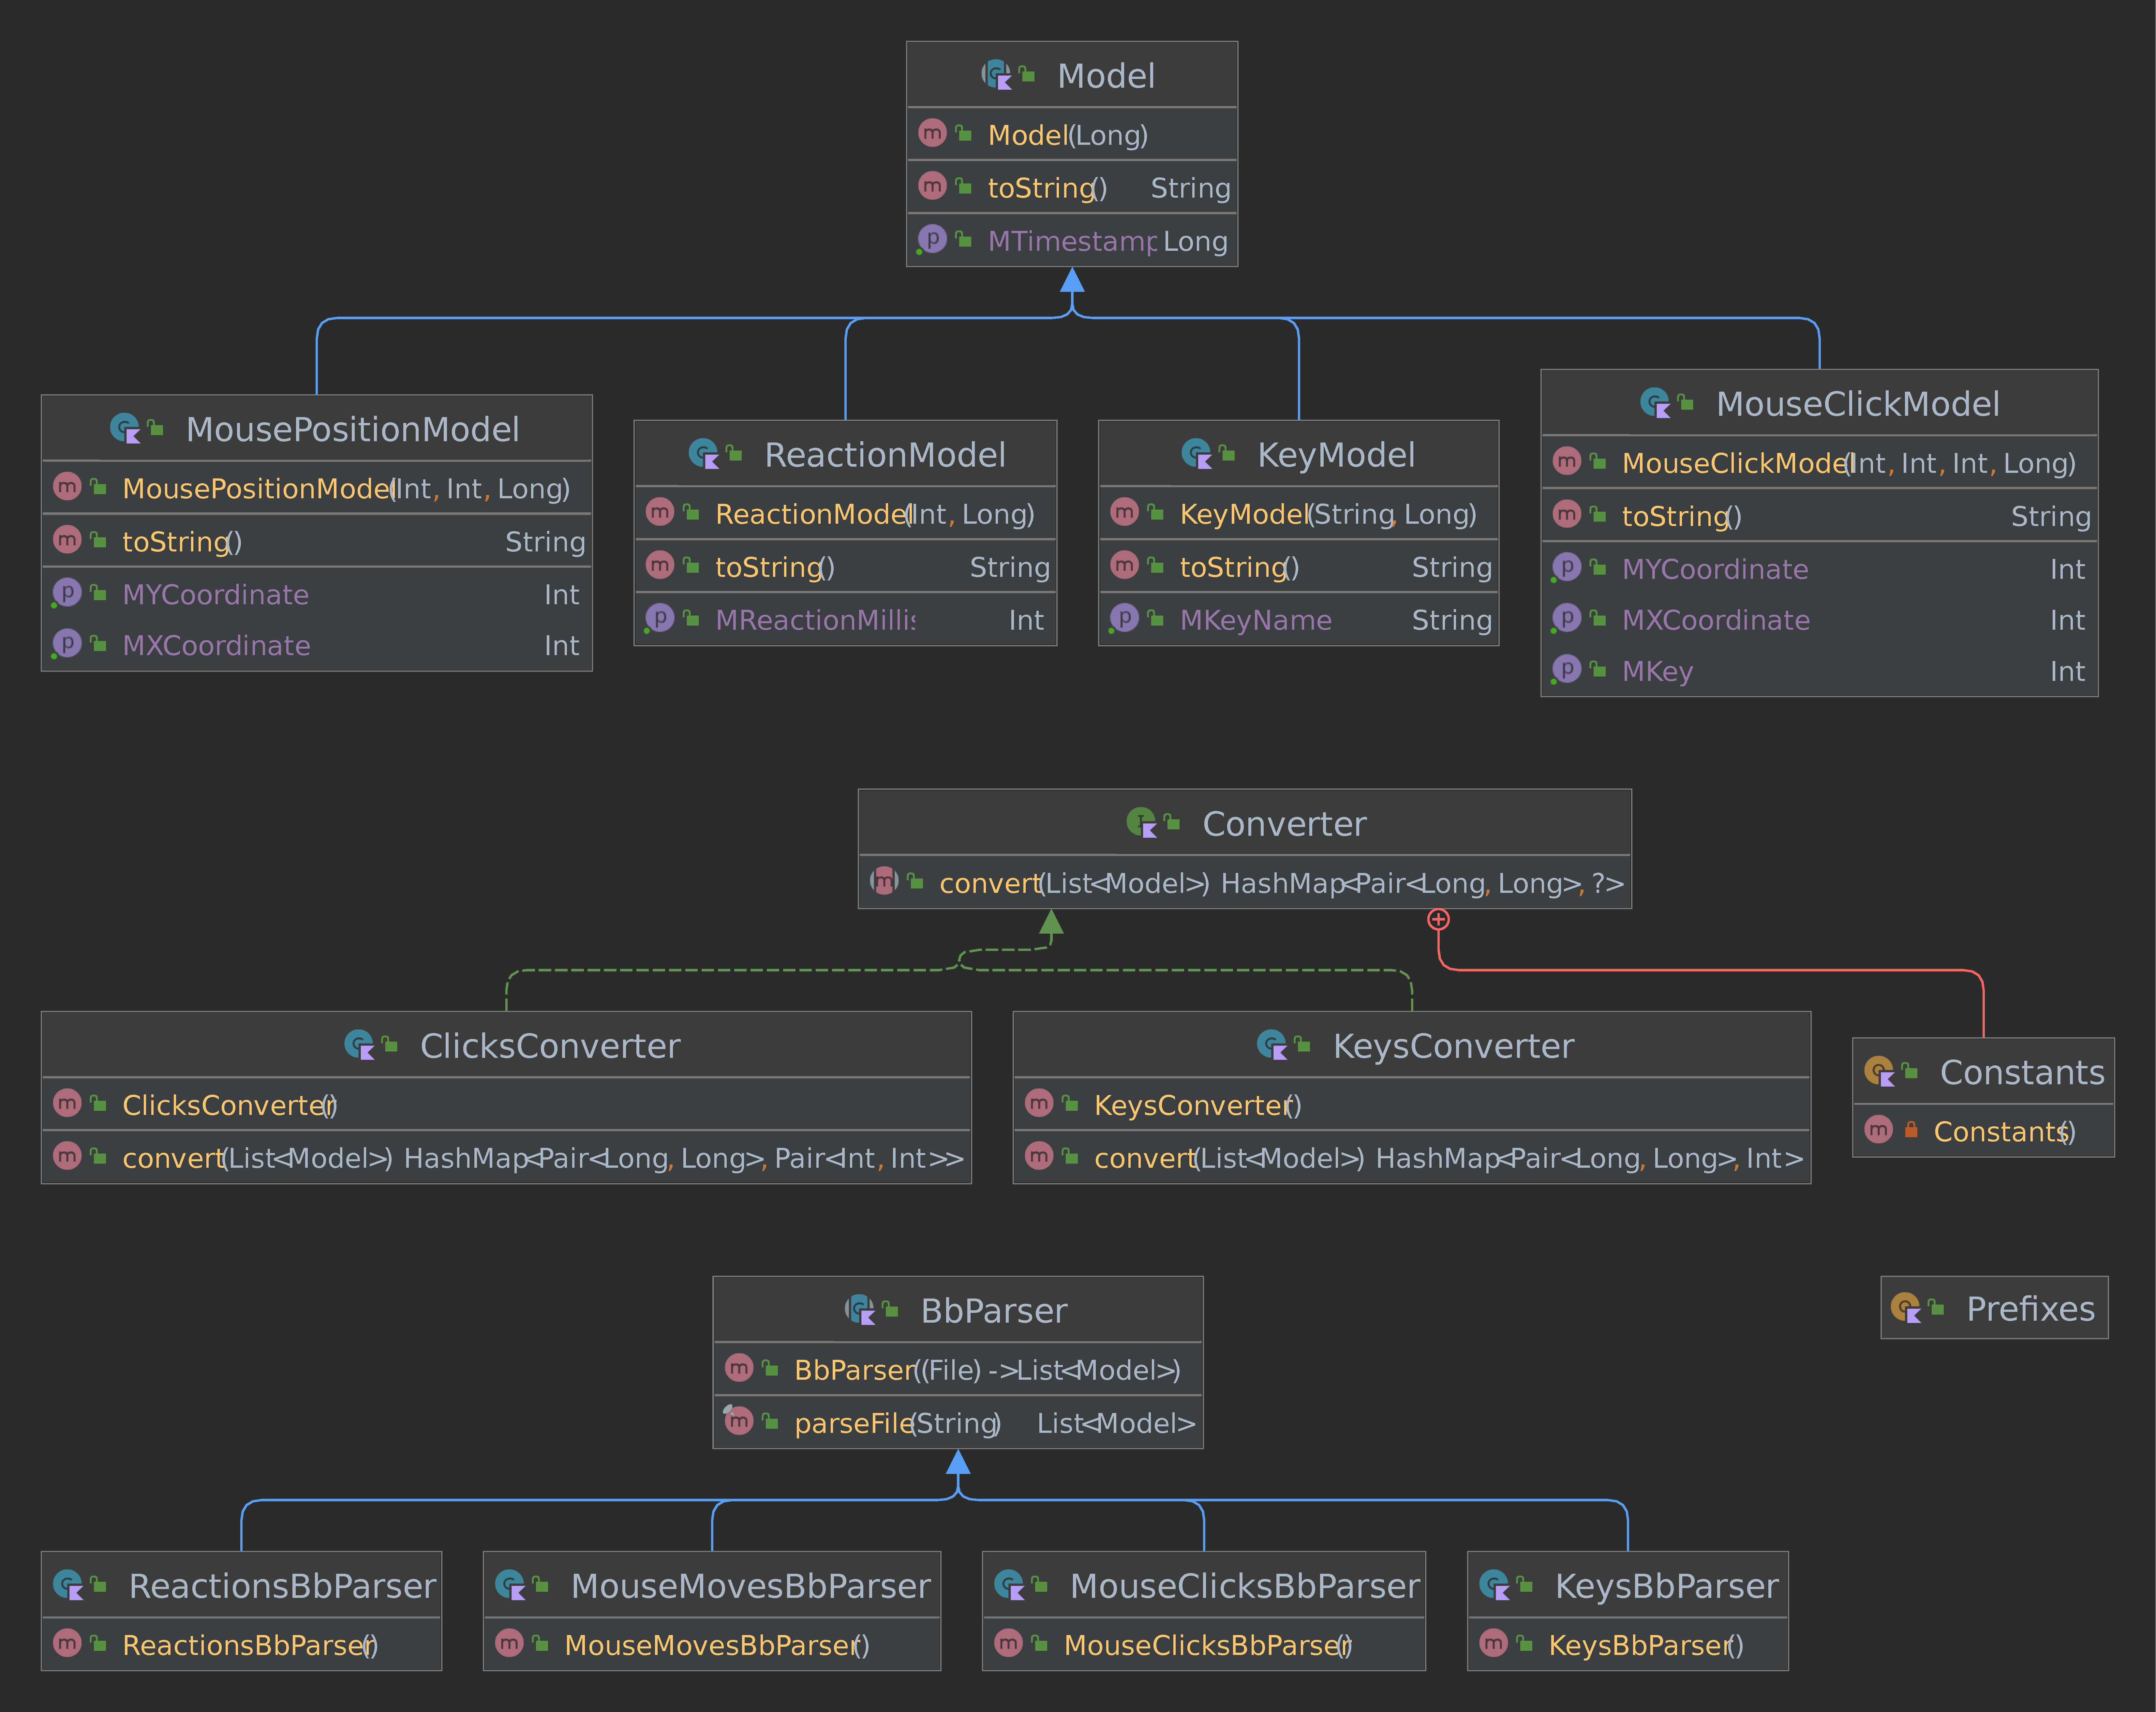
\includegraphics[width=\textwidth]{img/processing.pdf}
	\caption{Диаграмма классов модуля обработки данных.}
	\label{fig:processingUml}
\end{figure}

\subsubsection{Модуль анализа данных}
Данный модуль предназначен для анализа поступающих от оператора данных: кластеризации данных для модели и непосредственно текущей оценки усталости оператора.

Единственной библиотекой, используемой в модуле является The Commons Mathematics Library \cite{apachemath3}, из которой была взята реализация алгоритма кластеризации ``с-средних''.

\paragraph{Пакет analyze.clusterization \newline}

Данный пакет включает в себя утилиты для кластеризации данных, в нем представлен абстрактный класс Clusterer и его реализация BbClusterer, предоставляющий возможность определения нечетких кластеров по переданным данным. Также в пакете приведен класс точки для кластеризации, используемая библиотекой The Commons Mathematics Library. Реализация приведена в листингах \ref{lst:Clusterer} --- \ref{lst:BbClusterer}.

\lstinputlisting[
	caption={Файл Clusterer.kt},
	label={lst:Clusterer},
	language=kotlin
]{../BigBrother/src/main/kotlin/analyze/clusterization/Clusterer.kt}

\lstinputlisting[
	caption={Файл ClusterPoint.kt},
	label={lst:ClusterPoint},
	language=kotlin
]{../BigBrother/src/main/kotlin/analyze/clusterization/ClusterPoint.kt}

\lstinputlisting[
	caption={Файл BbClusterer.kt},
	label={lst:BbClusterer},
	language=kotlin
]{../BigBrother/src/main/kotlin/analyze/clusterization/BbClusterer.kt}

\paragraph{Пакет analyze.analyzers}

Данный пакет включает в себя анализаторы, позволяющие построить модель и оценивать состояние оператора с использованием различных способов предоставления данных. В листингах \ref{lst:Analyzer} и \ref{lst:BbAnalyzer} предоставлены абстрактный класс анализатора и его реализация для работы с файлами.

\lstinputlisting[
	caption={Файл Analyzer.kt},
	label={lst:Analyzer},
	language=kotlin
]{../BigBrother/src/main/kotlin/analyze/analyzers/Analyzer.kt}

\lstinputlisting[
	caption={Файл BbAnalyzer.kt},
	label={lst:BbAnalyzer},
	language=kotlin
]{../BigBrother/src/main/kotlin/analyze/analyzers/BbAnalyzer.kt}

\paragraph{Пакет analyze.fileAnalyzer}
Данный пакет предоставляет реализацию класса, позволяющего полноценно создать модель по заданным файлам и определить состояния оператора. Реализация представлена в листинге \ref{lst:BbFileAnalyzer}.

\lstinputlisting[
	caption={Файл BbFileAnalyzer.kt},
	label={lst:BbFileAnalyzer},
	language=kotlin
]{../BigBrother/src/main/kotlin/analyze/fileAnalyzer/BbFileAnalyzer.kt}

На рисунке \ref{fig:analyzerUml} предоставлена диаграмма классов модуля.

\begin{figure}[H]
	\centering
	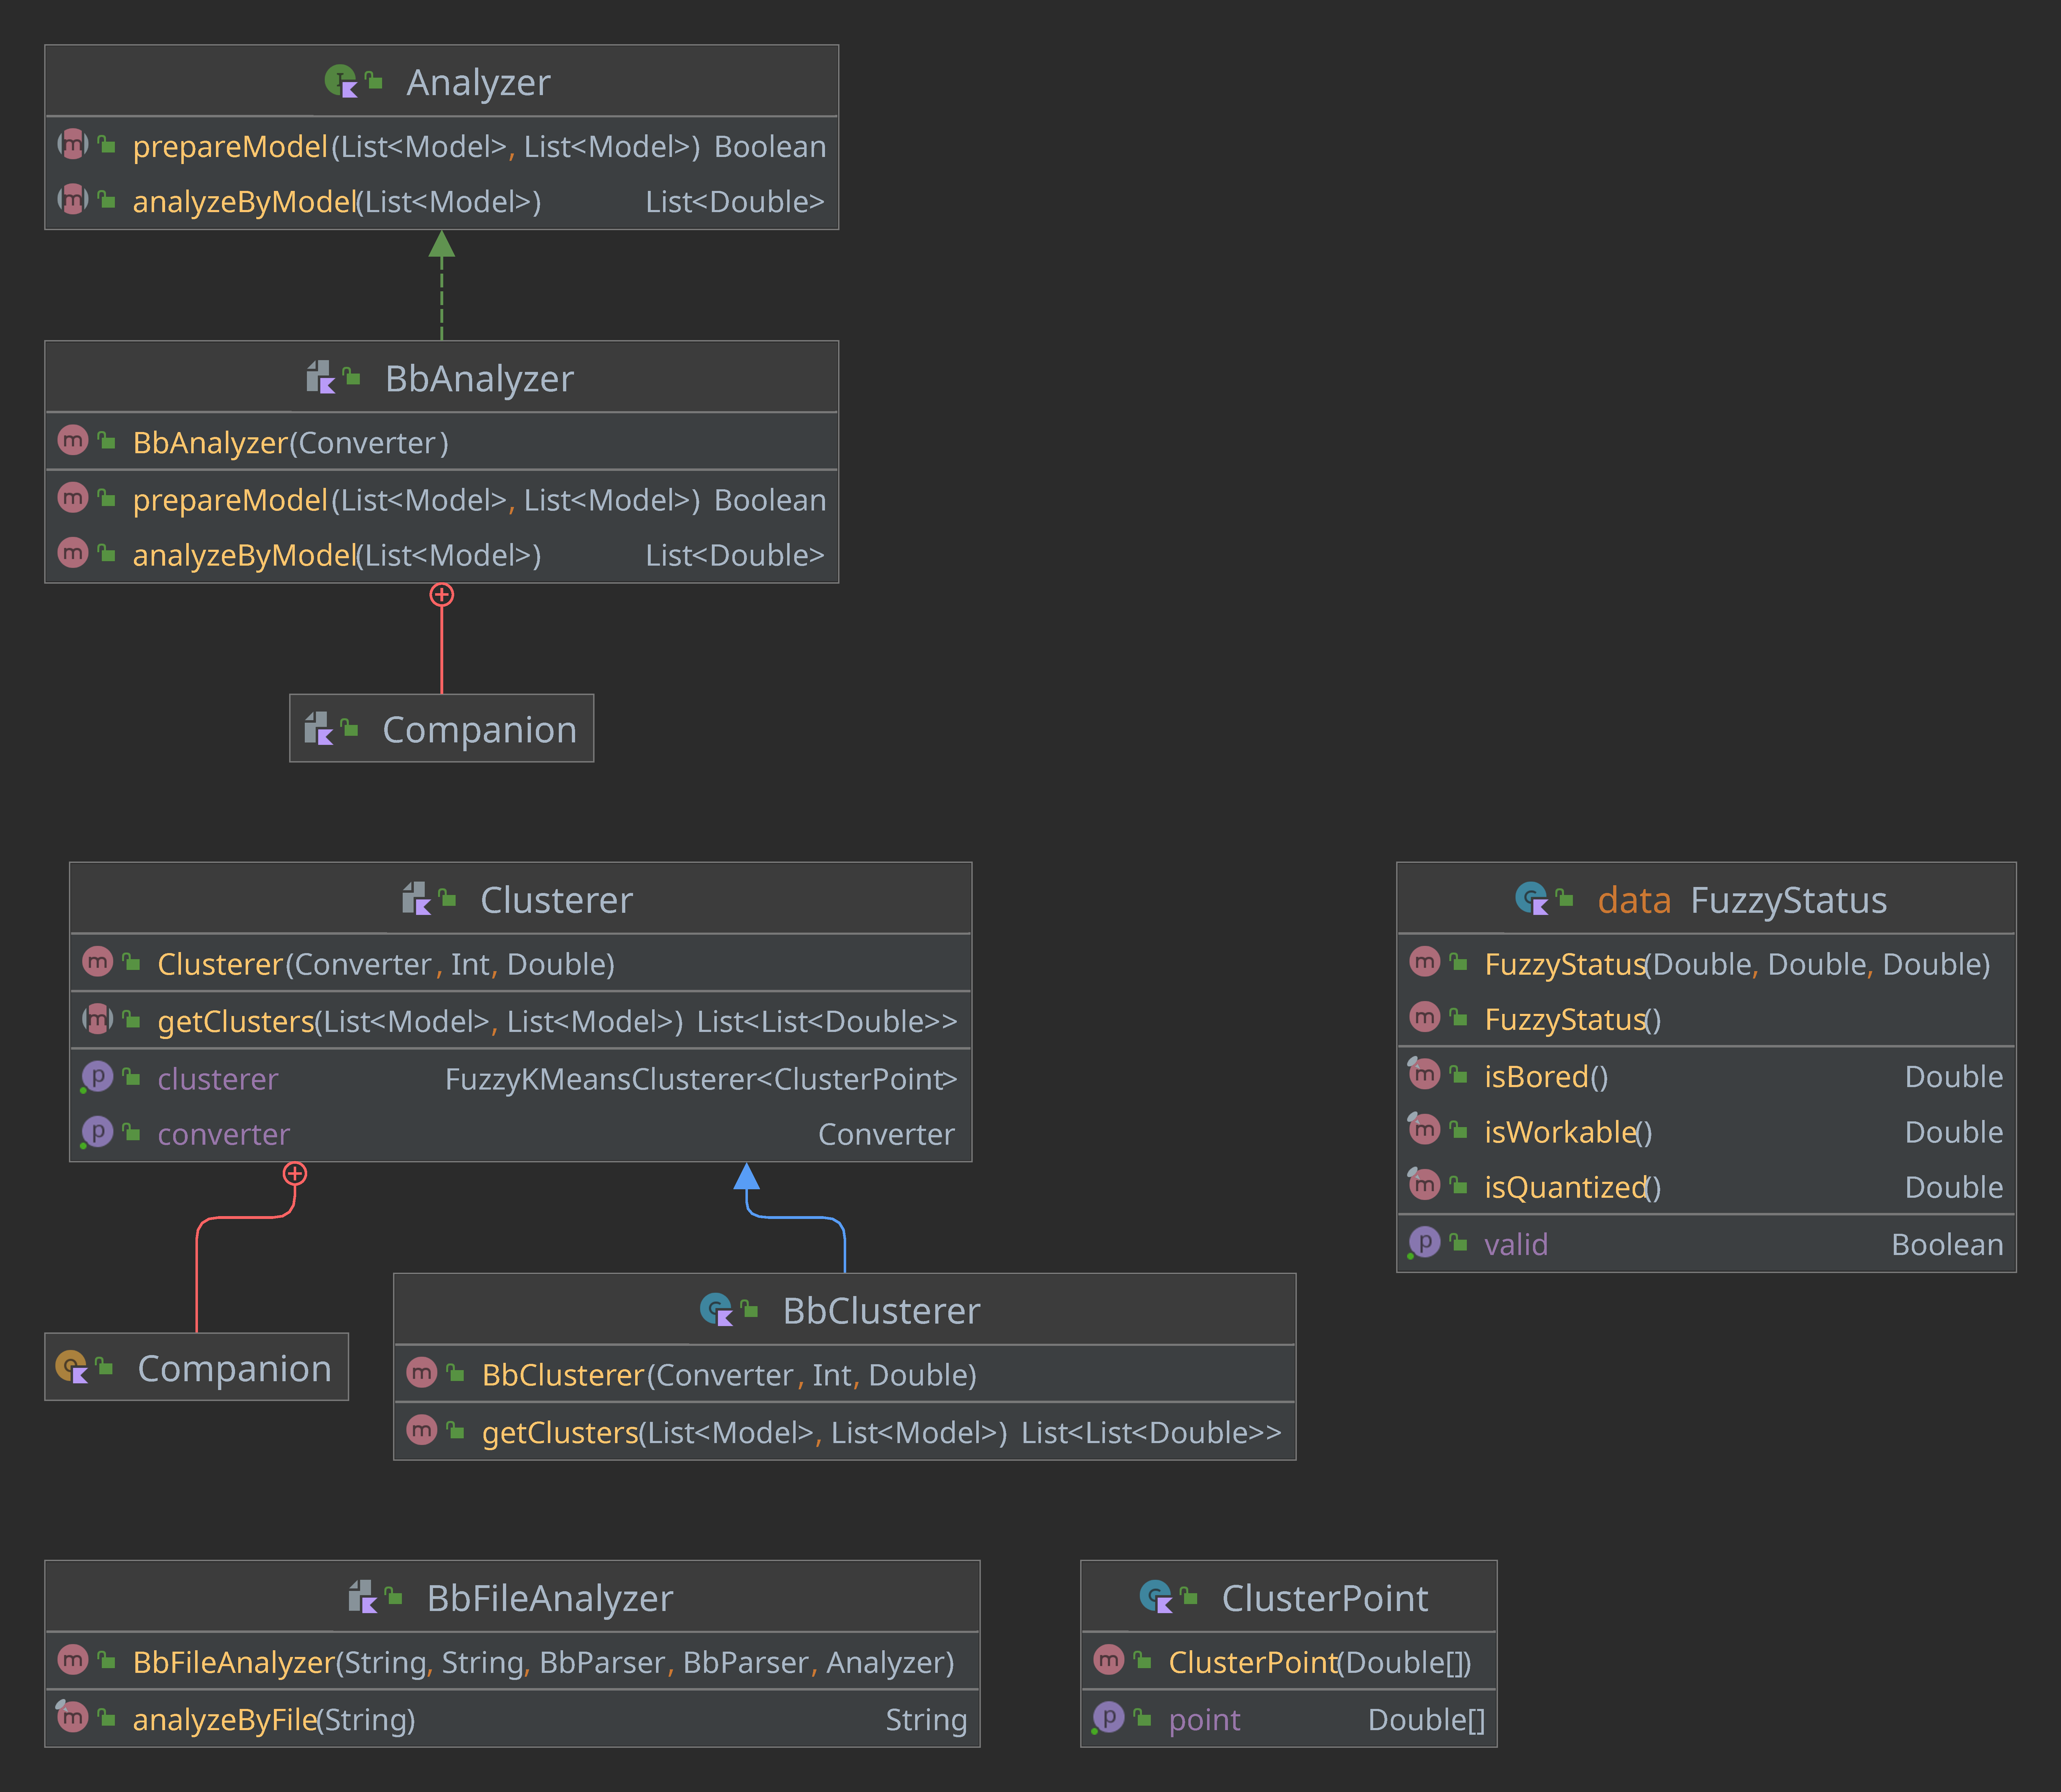
\includegraphics[width=\textwidth]{img/analyze.pdf}
	\caption{Диаграмма классов модуля анализа данных.}
	\label{fig:analyzerUml}
\end{figure}

\subsection{Развертывание системы}

